
\chapter{Programmable topotaxis of magnetic rollers in time-varying  fields$^\dag$}


\begin{center}
\vspace*{1\baselineskip}
\textbf{Abstract}
\end{center}
Time-varying uniform magnetic field can exert torque on ferromagnetic micro particles thereby driving their rotation motions. Such rotation motions can be hydrodynamically coupled to translation motions when the micro spheres are near a boundary. Here, time-varying (spatially uniform) magnetic fields are  programmed to navigate micro spheres' rolling motion on an inclined slope, showing gravitaxis behaviors (either downhill or uphill). A physical model is  built  to describe ferromagnetic micro particles' motions near a surface in a time-varying magnetic field. Then we introduce reverse design strategy to optimize the optimal magnetic field for navigating different behaviors of micro particles. Some preliminary experiment results are also shown for further investigation. 
 
\section{Introduction}
The autonomous navigation of active or driven particles within anisotropic environments is an essential capability in creating colloidal robots\cite{palagi2018bioinspired,han2018engineering} that operate without external supervision and control. Inspired by chemotactic bacteria that swim up (or down) gradients in the concentration of a chemoattractant (or repellant), colloidal motors can now direct their self-propelled motions in response to gradients in chemical concentrations,\cite{hong2007chemotaxis} magnetic potential,\cite{Kline2005} light intensity,\cite{dai2016programmable,lozano2016phototaxis} fluid velocity,\cite{Palacci2015,ren2017rheotaxis} fluid viscosity,\cite{liebchen2018viscotaxis} and gravitational potential.\cite{campbell2013gravitaxis,ten2014gravitaxis} Typically, these navigation strategies rely on gradient-driven torques to rotate anisotropic particles in a preferred orientation, thereby directing their motion---often by a different mechanism. For example, Janus spheres orient their denser hemisphere downward in a gravitational field to direct their self-phoretic propulsion upward against the gravity direction.\cite{campbell2013gravitaxis} Owing to their dependence on gradient-driven torques, these strategies are generally ineffective in weak gradients where other torques---for example, due to Brownian motion or self-propulsion---have a stronger influence on particle orientation.  Recently, we proposed a strategy to navigate weak gradients by using stimuli-responsive materials as high-gain sensors to inform the shape-directed motions of shape-shifting particles.\cite{dou2019autonomous} By carefully selecting the shape of the particle and its stimulus response, one can program autonomous motions in different directions relative to the gradient. More generally, particle shape\cite{brooks2018shape,sabrina2018shape,brooks2019shape} and composition\cite{lee2019directed} provide a rich design space with which to encode the desired behaviors of colloidal motors. However, the realization of these designs can present challenges in synthesizing complex anisotropic particles.
 
Alternatively, time-varying magnetic fields in three-dimensions (3D) provide an experimentally accessible design space, with which to direct complex motions of even simple particles. Rotating fields induce torques on magnetic particles,\cite{Janssen2009} which drive their rotation and translation near solid substrates due to hydrodynamic interactions.\cite{Swan2007} In this way, ferromagnetic spheres with residual magnetic moments\cite{Driscoll2017} as well as superparamagnetic particles with anisotropic susceptibilities\cite{Tierno2008} are driven to “roll” on planar substrates as directed by the external field. Recent work on these colloidal rollers has focused on their collective behaviors within dynamic assemblies such as flocks,\cite{Kaiser2017} swarms,\cite{Xie2019} worms,\cite{Martinez-Pedrero2015} wheels,\cite{Tasci2016} and critters.\cite{Driscoll2017} At the level of individual particles, there remain interesting questions on the influence of particle shape\cite{Zhang2010} and surface topography\cite{Yang2019} on propulsion dynamics in simple time-periodic fields (e.g., oscillating, rotating, precessing).
 
Here, we investigate the use of complex time-varying fields to inform the dynamics of ferromagnetic spheres moving in a viscous fluid above an inclined plane (Fig.~XXX). We show how designed fields can be used to encode steady particle motions up (or down) the inclined surface \emph{without} knowledge of its orientation or the particle’s location. Importantly, the applied field does not instruct the particle on which direction to move but rather on how to respond to local variations in the particle environment. As a result, the same field can drive multiple independent particles to move simultaneously in different directions as determined by local gradients in the surface topography.  We refer to these gradient-driven motions as \emph{topotaxis} by analogy to the biological phenomenon of the same name.\cite{Park2018} Our results are based on a dynamical model that considers the time-varying magnetic torques on the particle and its resulting motion through the fluid at low Reynolds number. Using a two-timing perturbation scheme, we develop analytical approximations for the drift velocity accurate to first order in the incline angle and to second order in the driving frequency.   This analysis reveals that topotactic motions rely on differences in the hydrodynamic resistance to rotation about axes parallel and perpendicular to the plane. Using numerical simulations, we identify complex driving fields that maximize the speed of gradient-driven motion up (or down) the inclined surface.  Our results demonstrate how complex time-varying fields can be used to both power and instruct the autonomous behavior of colloidal particles in anisotropic environments.

%Living cells or bacteria show the fantastic ability of navigation called chemotaxis\cite{alon1999robustness,adler1975chemotaxis}. The chemotactic microorganism can trace the very limited information in  a complex micro noisy environment for the food source or suitable living space\cite{keller1971model}. This kind of navigation behavior in the living system is also highly desirable in synthetic micro swimmers or active matter systems \cite{patteson2016active}. Only with efficient and accurate navigation behaviors in a complex environment, synthetic micro swimmers can fully extend their engineering applications such as drug delivery and surgery\cite{de2017micromotor,xu2018sperm}. Although lots of synthetic  micro swimmers can do autonomous directed propulsion \cite{yan2016reconfiguring,lee2019directed,baker2019shape}, their motions are biased by  external field or inherent asymmetry instead of information from environment. Thereby, it is essential to introduce new strategies for micro swimmers so that micro swimmers can interact with the environment and show navigation behaviors.  

%The suffix "-taxis" in chemotaxis refers to the motion following a physical or chemical properties gradient. Recently, some experimental or theoretical attempts have been reported to make "taxis" synthetic microswimmers. Phototaxis particles can see the gradient of light due to the local thermal gradient near the colloid particle\cite{yu2019phototaxis,dai2016programmable,lozano2016phototaxis,chen2017light}; gravitaxis swimmers can swim against the gravity \cite{campbell2013gravitaxis,ten2014gravitaxis}; rheotaxis swimmers can orient their direction autonomously against the fluid flow\cite{Palacci2015,ren2017rheotaxis,brosseau2019relating}; bio-mimic chemotaxis swimmers can sense the local gradient of chemical species and move towards the source or drain of chemicals\cite{dou2019autonomous}; visoctaxis particles can swim towards the fluid regions of higher or lower viscosity\cite{liebchen2018viscotaxis}. However, these approaches all depend on the fabrication of microswimmers with some particular asymmetric geometry--colloidal particles of anisotropic shapes or components. Different navigation directions in a different environment can only be achieved by redesigning the particles, which is a complex and non-efficient process. Less research has been shown to navigate an isotropic particle's taxis behaviors. A more programmable and tangible mechanism is needed to navigate a large amount of particles autonomously \cite{dou2019autonomous}.

%Here, we propose a new gravitaxis mechanism that uses a programmed time-varying magnetic field on isotropic magnetic micro spheres placed on an inclined surface. Microspheres in fluid rolling on a surface can couple the rotation motion to translation motion via hydrodynamics\cite{galvin2001time,rashidi2016theoretical}. Ferromagnetic micro spheres with permanent magnetic dipole  can response to the external  magnetic showing different rolling dynamics \cite{helgesen2019propulsion,helgesen2018magnetic}. The external magnetic field provides a rich programmed design space to control the dynamics of magnetic rollers. In this chapter, we show that programmed the external magnetic fields exerted on  micro rollers can achieve autonomous gravitaxis (either downhill or uphill) behaviors on an inclined slope. A physical model is described first to simulate the motions of magnetic rollers. Then we explore the design space for the magnetic field  and optimize the magnetic field, which can actuate the desired navigation trajectories of micro rollers.




%%%%%%%%%%%%%%%%%%%%%%%%%%%%%%%
%%%%%%%%%%%%%%%%%%%%%%%%%%%%%%%
%%%%%%%%%%%%%%%%%%%%%%%%%%%%%%%
\section{Ferromagnetic Rollers}

We consider a magnetic sphere with radius $a$ and permanent magnetic moment $\ve{m}$ moving through a viscous fluid at a fixed height above a solid plane under the influence of a time-varying magnetic field $\ve{B}(t)$. In a uniform field, the particle experiences a magnetic torque, $\ve{L}=\ve{m}\times\ve{B}(t)$, but no magnetic force, $\ve{F}=0$. In the absence of inertial effects (i.e., at low Reynolds number), the magnetic force and torque on the particle are balanced by the hydrodynamic force and torque, which are linearly related to the particle's linear velocity $\ve{U}$ and angular velocity $\veS{\Omega}$ as
\begin{equation}
    \begin{bmatrix} \ve{F} \\ \ve{L} \end{bmatrix} = \begin{bmatrix} A & \tilde{B} \\ B & C \end{bmatrix}  \begin{bmatrix} \ve{U} \\ \veS{\Omega} \end{bmatrix} \label{eq:dynamics}
\end{equation}
where $A$, $B$, $\tilde{B}$, and $C$ are components of the hydrodynamic resistance matrix.  

For a solid sphere above a solid plane normal to the $z$-direction, the components of the resistance tensor have the form
\begin{align}
    A &=  6\pi \eta a \begin{bmatrix} 
        Y_A & \cdot & \cdot \\
        \cdot & Y_A & \cdot \\
        \cdot & \cdot & X_A  \end{bmatrix}
    \\
    B=-\tilde{B}&= 6\pi \eta a^2 \begin{bmatrix} 
        \cdot & Y_B & \cdot \\
        -Y_B & \cdot & \cdot \\
        \cdot & \cdot & \cdot  \end{bmatrix}
    \\
    C &= 6\pi \eta a^3 \begin{bmatrix} 
        Y_C & \cdot & \cdot \\
        \cdot & Y_C & \cdot \\
        \cdot & \cdot & X_C 
    \end{bmatrix} 
\end{align}
where $\eta$ is the fluid viscosity. The coefficients $Y_A$ and $Y_B$ describe, respectively, the dimensionless force and torque on a sphere translating parallel to a solid planar surface.\cite{ONeill1964a} The coefficient $Y_C$ describes the torque on a sphere rotating about an axis parallel to the surface.\cite{Dean1963} The coefficient $X_A$ describes the force on a sphere translating perpendicular to the surface.\cite{Brenner1961a}  Finally, $X_C$ describes the torque on a sphere rotating about an axis perpendicular to a the surface.\cite{Jeffrey1915} These coefficients depend only on the surface separation, $\delta=z_p-a$, scaled by the particle radius $a$.

Substituting the above expressions for the resistance tensor, the linear velocity $\ve{U}$ and angular velocity $\veS{\Omega}$ can be expressed explicitly in terms of the magnetic torque as
\begin{align}
    6\pi\eta a^2 \ve{U} &= \frac{Y_A}{Y_A Y_C - Y_B^2}\begin{bmatrix} 
        \cdot & \kappa & \cdot \\
        -\kappa & \cdot & \cdot \\
        \cdot & \cdot & \cdot  \end{bmatrix} \ve{L}  \label{eq:U}
    \\
    6\pi\eta a^3 \veS{\Omega} &= \frac{Y_A}{Y_A Y_C - Y_B^2}\begin{bmatrix} 
        1 & \cdot & \cdot \\
        \cdot & 1 & \cdot \\
        \cdot & \cdot & \lambda  \end{bmatrix} \ve{L} \label{eq:W}
\end{align}
where $\kappa = Y_B/Y_A$ and $\lambda=(Y_A Y_C -Y_B^2)/(Y_A X_C)$. These dynamics imply that the particle velocity normal to the planar substrate is identically zero (i.e., $U_z=0$). We therefore assume that the surface separation $\delta$ and the resistance coefficients are constant throughout the particle's dynamics.  For a surface separation of $\delta = 0.01 a$, the dimensionless parameters are $\kappa = 0.108$ and $\lambda=1.87$ (see Supporting Figure XXX for plots of $\kappa$ and $\lambda$ vs.~$\delta/a$).  

Our present analysis neglects the effects of gravity and of Brownian motion. A gravitational force normal to the surface is implicit in our assumption of a constant surface separation $\delta$. Gravity-driven motions tangent to the surface are assumed to be negligible compared to those induced by the magnetic field. As detailed below, this assumption is valid when $M g a / m B_0 \ll XXX$, where $M$ is the buoyant mass of the particle, and $g$ is the acceleration due to gravity. Similarly, we assume that magnetic torques are sufficiently large as to neglect Brownian motion, which is appropriate when $k_B T / m B_0 \ll 1$ where $k_BT$ is the thermal energy. The validity of these assumptions is discussed further in the Supporting Information.

%%%%%%%%%%%%%%%%%%%%%%%%%%%%%%%%%%
\subsection{Non-dimensionalization}

To facilitate both numerical solution and analytical analysis of the particle dynamics, it is convenient to introduce dimensionless variables using the following scales
\begin{align}
    \text{field:  } & B_0
    \\
    \text{torque:  } &  mB_0
    \\
    \text{length:  } & a
    \\
    \text{time:  } & \frac{6\pi \eta a^3 (Y_A Y_C-Y_B^2)}{m B_0 Y_A}  
\end{align}
Here, $B_0$ is the characteristic magnitude of the applied field. In dimensionless form, the dynamical equations (\ref{eq:U}) and (\ref{eq:W}) depend on the  two constant parameters $\kappa$ and $\lambda$ along with the time-varying magnetic field $\ve{B}(t)$. Below, we use the same notation to refer to dimensionless quantities, which corresponds to setting the characteristic scales to unity in the dynamical equations (\ref{eq:U}) and (\ref{eq:W}) (e.g., $a\rightarrow 1$).

%%%%%%%%%%%%%%%%%%%%%%%%%%%%%%%%%%
\subsection{Euler Angle Dynamics}

The dynamics of equations (\ref{eq:U}) and (\ref{eq:W}) are solved numerically to determine the particle position $\ve{x}_{\p}(t)$ and its orientation parameterized by the Euler angles  $\ve{u}=[\phi,\theta,\psi]^T$. At each point in time, the magnetic torque $\ve{L}$ expressed in the surface coordinate system (Fig.~\ref{fig:Coordinates}) is given by 
\begin{equation}
    \ve{L} = (R_{313}^{T}(\ve{u})~\ve{m}'')\times \ve{B}(t) \label{eq:Lm}
\end{equation}
where $\ve{m}''=[0,0,1]^T$ is the constant magnetic moment expressed in the particle coordinate system, and $R_{313}(\ve{u})=R_3(\phi)R_1(\theta)R_3(\psi)$ is the rotation matrix for the $(3,1,3)$ sequence of Euler angles.\cite{Diebel2006} Given the torque $\ve{L}$, the linear velocity $\ve{U}$ and angular velocity $\veS{\Omega}$ are given by equations (\ref{eq:U}) and (\ref{eq:W}). Starting from initial conditions $\ve{x}_p(0)$ and $\ve{u}(0)$, the position and orientation evolve as 
\begin{align}
    \dot{\ve{x}}_p &= \ve{U} \label{eq:position}
    \\
    \dot{\ve{u}} &= \frac{1}{s_{\theta}}\begin{bmatrix} 
     s_{\psi} & -c_{\psi} & 0
     \\
     s_{\theta} c_{\psi} & s_{\theta} s_{\psi} & 0
     \\
     -s_{\psi}c_{\theta} & c_{\psi}c_{\theta} & s_{\theta}
     \end{bmatrix} \cdot \veS{\Omega}
\end{align}
with $c_x =\cos(x)$ and $s_x=\sin(x)$.\cite{Diebel2006} The resulting dynamical equations for the particle orientation can be simplified as
\begin{align}
    \dot{\phi} &= -\cot \theta (B_x\cos\psi +B_y\sin\psi)
    \\
    \dot{\theta} &=  -\cos\theta (B_y \cos\psi - B_x \sin\psi) - B_z\sin\theta \label{eq:theta}
    \\
    \dot{\psi} &= \tfrac{1}{2} \left((1+\lambda) +(1-\lambda)\cos2\theta \right) \csc\theta (B_x \cos \psi + B_y\sin\psi ) \label{eq:psi}
\end{align}
Note that the dynamics of the angles $\theta$ and $\psi$ can be solved independently of $\phi$.  This simplification follows from the fact that there is no torque on the particle about the axis of its magnetic moment. Similarly, the particle velocity in the plane of the substrate can be expressed as
\begin{align}
    U_x = \kappa (B_x \cos \theta -  B_z \sin \psi \sin\theta) \label{eq:Ux}
    \\
    U_y = \kappa (B_y \cos\theta + B_z \cos\psi \sin\theta ) \label{eq:Uy}
\end{align}
Equations (\ref{eq:theta})--(\ref{eq:Uy}) can be integrated numerically to determine the motion of the particle in the prescribed magnetic field $\ve{B}(t)$.

\begin{figure}
    \centering
    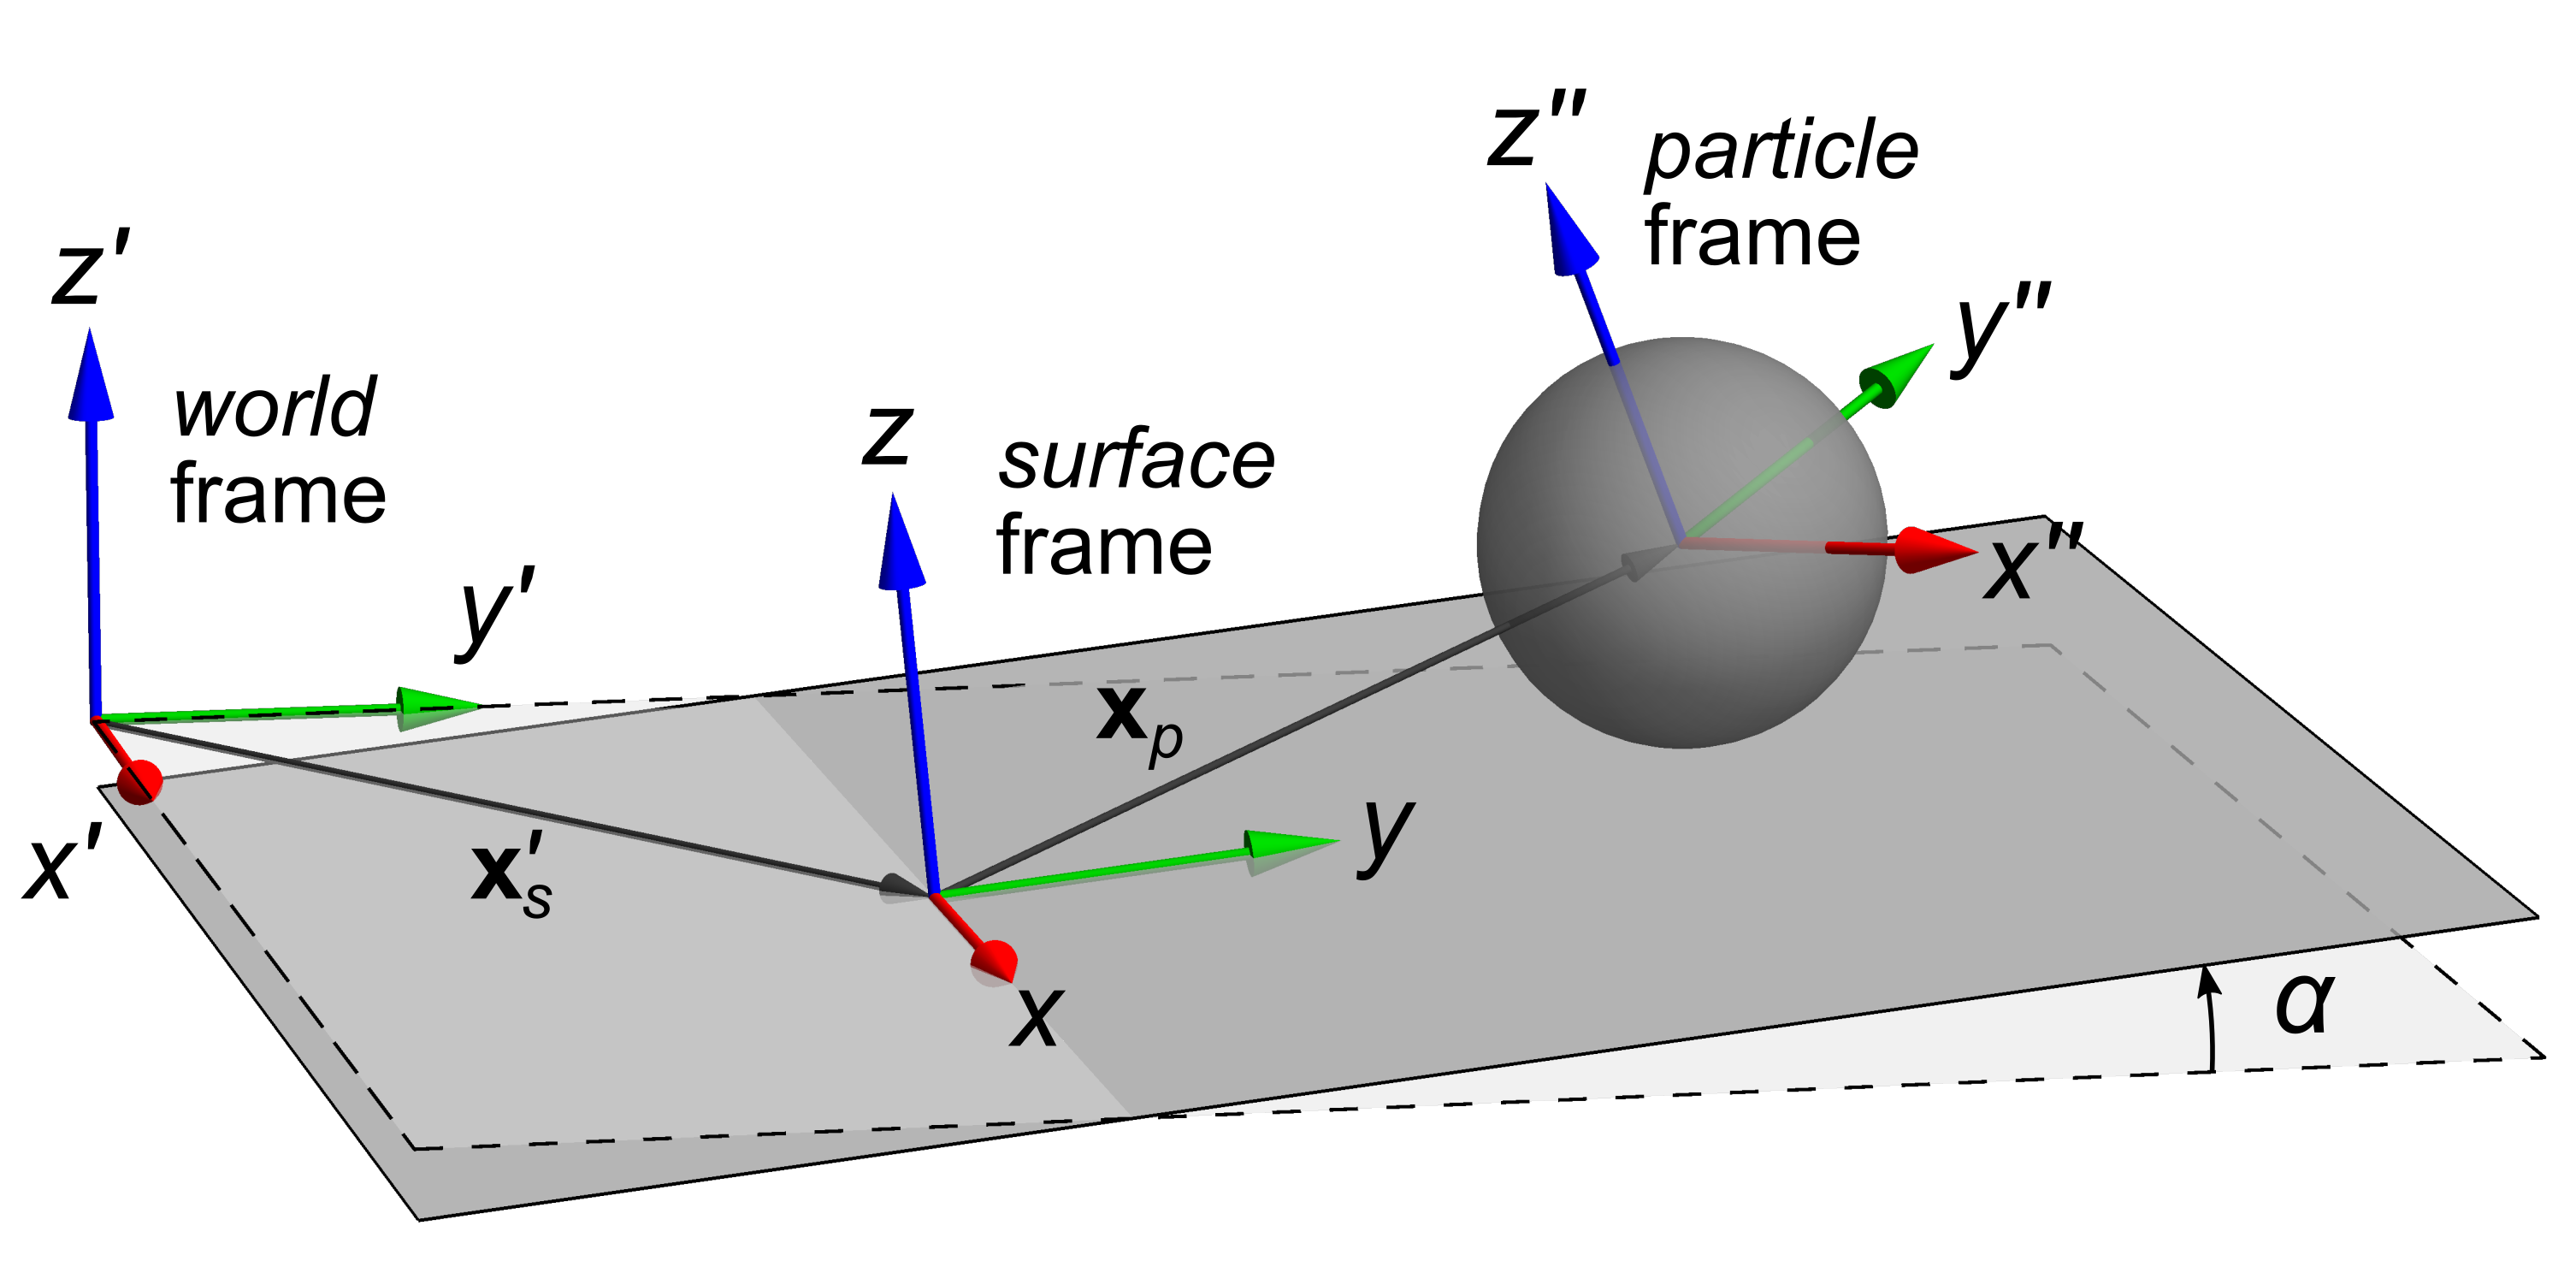
\includegraphics[width=8.5cm]{figures/5Coordinates.png}
    \caption{Three coordinate systems used to describe particle motion.\cite{Diebel2006}  A point $\ve{x}$ in the \emph{surface} coordinates is related to the same point $\ve{x}'$ in the \emph{world} coordinates as $\ve{x}=R_1(\alpha) (\ve{x}'-\ve{x}'_s)$. Here, the matrix $R_1(\alpha)$ denotes rotation about the $x$-axis by an angle $\alpha$; the vector $\ve{x}'_s$ is the origin of the surface coordinates expressed in the world coordinates. Similarly, a point $\ve{x}''$ in the \emph{particle} coordinates is related to the same point $\ve{x}$ in the \emph{surface} coordinates as $\ve{x}''=R_{313}(\ve{u})(\ve{x}-\ve{x}_p)$ where $R_{313}(\ve{u})=R_3(\phi)R_1(\theta)R_3(\psi)$ is the rotation matrix for the (3,1,3) sequence of Euler angles $\ve{u}=[\phi,\theta,\psi]^T$. }
    \label{fig:Coordinates}
\end{figure}

%%%%%%%%%%%%%%%%%%%%%%%%%%%%%%%%%%
%%%%%%%%%%%%%%%%%%%%%%%%%%%%%%%%%%
\subsection{Two-Timing Perturbation Solution}

For time-periodic magnetic fields of frequency $\omega$, the particle dynamics can be approximated using a perturbation expansion based on \emph{two-timing},\cite{Strogatz2015} where the dimensionless frequency is treated as the small parameter. Physically, this parameter represents the ratio between the driving frequency of the applied field and the relaxation rate of the magnetic particle. The assumption that $\omega\ll 1$ implies that relaxation is fast, such that the particle's magnetic moment aligns closely with the field. Under these conditions, we can introduce two time variables: a slow time, $T=\omega t$, corresponding to the driving field and a fast time, $\tau=t$, corresponding to particle relaxation. The solution to equations (\ref{eq:theta})--(\ref{eq:Uy}) can then be expanded as
\begin{align}
    \theta(t,\omega) &= \theta_0(\tau,T) + \omega \theta_1(\tau,T) + \omega^2 \theta_2(\tau,T) + O(\omega^3) \label{eq:thetaPower}
    \\
    \psi(t,\omega) &= \psi_0(\tau,T) + \omega \psi_1(\tau,T) + \omega^2 \psi_2(\tau,T) + O(\omega^3) \label{eq:psiPower}
    \\
    \ve{U}(t,\omega) &= \omega \ve{U}_1(\tau,T) + \omega^2 \ve{U}_2(\tau,T) + O(\omega^3) \label{eq:UPower}
\end{align}
where $\tau$ and $T$ and treated as independent variables. Substituting these expansions into the governing equations and collecting like powers in $\omega$, we obtain a hierarchy of perturbation equations that can be solved sequentially. We are primarily interested in the slow time dynamics of the particle over one cycle of the oscillation period; we therefore focus on the limit as $\tau\rightarrow\infty$ in which the fast processes have fully relaxed.

At the periodic steady-state ($\tau\rightarrow\infty$), the average velocity $\langle\ve{U}\rangle$ of the particle is given by the following integral of the slow time over one oscillation cycle
\begin{equation}
    \langle\ve{U}\rangle = \frac{1}{2\pi} \int_0^{2\pi} \ve{U}(\infty, T) dT
\end{equation}
where the components of the velocity are given by equations (\ref{eq:Ux}) and (\ref{eq:Uy}).  Substituting the perturbation expansion (\ref{eq:UPower}), the average velocity can be expanded as
\begin{equation}
    \langle\ve{U}\rangle = \omega \langle\ve{U}_1\rangle + \omega^2 \langle\ve{U}_2\rangle + O(\omega^3) \label{eq:averageU}
\end{equation}
Note that the zeroth order contributions are identically zero as there is no motion in the limit of zero frequency. In Appendix A, we derive expressions for the the average velocity as a function of the applied field $\ve{B}(T)$.

%%%%%%%%%%%%%%%%%%%%%%%%%%%%%%%
%%%%%%%%%%%%%%%%%%%%%%%%%%%%%%%
%%%%%%%%%%%%%%%%%%%%%%%%%%%%%%%
\subsection{Topotaxis on an Inclined Surface}

We now consider the dynamics of a ferromagnetic roller on an inclined surface subject to a time-periodic magnetic field. To apply the results of the previous section, we make use of three coordinate systems: (1) the \emph{surface} coordinate, (2) the \emph{world} coordinate, and (3) the \emph{particle} coordinate (Fig.~\ref{fig:Coordinates}).  The solid plane is located at $z=0$ in the surface coordinate; the gravity vector is $\ve{g}'=[0,0, -g]^T$ in the world coordinate.  The  magnetic field vector $\ve{B}'(T)$ in the world coordinate is related to the same vector $\ve{B}(T)$ in the surface coordinate as $\ve{B}(T)=R_1(\alpha)\ve{B}'(T)$, where the matrix $R_1(\alpha)$ describes a coordinate rotation about the $x$-direction by an angle $\alpha$ (Fig.~\ref{fig:Coordinates}). For small angles ($\alpha\ll 1$), equation (\ref{eq:averageU}) for the average velocity can be expanded in powers of $\alpha$ as 
\begin{align}
\begin{split}
    \langle\ve{U}\rangle &= \omega( \langle\ve{U}_{10}\rangle + \alpha \langle\ve{U}_{11}\rangle + O(\alpha^2) ) 
    \\
    &+ \omega^2( \langle\ve{U}_{20}\rangle + \alpha \langle\ve{U}_{21}\rangle + O(\alpha^2) ) + O(\omega^3)
\end{split}
\end{align}
where the components of the velocity are determined by the applied field $\ve{B}'(T)$. By carefully selecting the field, one can drive particle motions in a particular direction relative to that of the inclined surface.  

%%%%%%%%%%%%%%%%%%%%%%%%%%%%%%%
%%%%%%%%%%%%%%%%%%%%%%%%%%%%%%%
%%%%%%%%%%%%%%%%%%%%%%%%%%%%%%%
\section{Results \& Discussion}

We turn now to the following design problem: what time-periodic magnetic field $\ve{B}'(T)$ will drive steady particle motion up (or down) an inclined surface?  Importantly, the direction of the incline is not known \emph{a priori}; the same field should drive ``uphill'' motions regardless of which direction is ``up''.  For multiple particles moving independently in a common field $\ve{B}'(T)$, the motion of each particle should be directed by the \emph{local} incline of the surface; the same field should drive different particles in different directions depending on the local surface topography. We address this design problem by two complementary approaches---one model-driven, another data-driven---and discuss their respective merits in light of this and other design challenges posed by colloidal robotics. Common to both approaches is the use of symmetry arguments to prevent undesired motions and constrain the design space of possible fields $\ve{B}'(T)$.  

%%%%%%%%%%%%%%%%%%%%%%%%%%%%%%%
%%%%%%%%%%%%%%%%%%%%%%%%%%%%%%%
\subsection{Rotational Symmetry}

We aim to drive steady particle motions up inclined surfaces: in the absence of an incline, there should be zero time-averaged motion.  We can enforce this condition by selecting external fields $\ve{B}'(T)$ with $m$-fold rotational symmetry about the $z'$ axis.  Specifically, we require that the applied field satisfy the condition
\begin{equation}
    R_3(\varphi_m) \ve{B}'(T) = \ve{B}'(T-\varphi_m) \label{eq:rotation}
\end{equation}
where $R_3(\varphi_m)$ describes a coordinate rotation about the $z'$-axis by an angle $\varphi_m=2\pi/m$ for a specified integer $m\geq3$. This condition implies that the rotation of the field by an angle $\varphi_m$ is equal to a shift in phase of $\varphi_m$.  

As a result of this symmetry, contributions to the average velocity at zeroth order in the angle $\alpha$ are identically zero (Appendix B)
\begin{equation}
    \langle\ve{U}_{10}\rangle = \langle\ve{U}_{20}\rangle = 0 \label{eq:alpha0}
\end{equation}
Although intuitive, this result is not guaranteed to apply at higher orders in the frequency $\omega$. It is possible that certain fields with rotational symmetry could drive steady particle motions on level surfaces ($\alpha=0$) at high frequencies; however, we did not observe such symmetry-breaking motions here.

At first order in $\alpha$, fields with rotational symmetry can drive motions perpendicular to the gradient direction at first order in the frequency $\omega$; however, motions parallel to the gradient direction do not appear until second order in $\omega$. For the scenario in Figure \ref{fig:Coordinates}, the leading order contribution to particle motion is
\begin{equation}
    \langle \ve{U}_{11}\rangle = \langle U_x^{(11)}\rangle \ve{e}_{x}  \label{eq:alpha1}
\end{equation}
which is perpendicular to the gradient direction (Appendix B). This result is potentially problematic: we would prefer the leading order contribution to describe desired motions up (or down) the gradient.  Recognizing this issue, we can use the model to design fields that eliminate such undesired motions.

%%%%%%%%%%%%%%%%%%%%%%%%%%%%%%%
%%%%%%%%%%%%%%%%%%%%%%%%%%%%%%%
\subsection{Model-driven Design}

For the present problem, it is possible to identify time-periodic magnetic fields that (1) prohibit undesired motions perpendicular to the gradient direction, and (2) offer control over the direction and speed of desired motions parallel to the gradient direction.  One such field is given by 
\begin{equation}
    \ve{B}'(T) = \begin{bmatrix} \cos \chi(T) \sin(m T) \\ \sin \chi(T) \sin(m T) \\ \cos(m T) \end{bmatrix} \label{eq:field}
\end{equation}
where $m\geq3$ is an integer that specifies the order of rotational symmetry, and the angle $\chi(T)$ is given by 
\begin{equation}
    \chi(T) = T - \frac{b}{m}\cos(m T)+ \frac{1}{4 m}\left(1+\sqrt{\lambda}\right)^2 \sin(2 m T)
\end{equation}
where $b$ is free parameter.  This field has a constant magnitude but time-varying orientation.  It satisfies the rotational symmetry constraint of equation (\ref{eq:rotation}).  Moreover, it is designed to eliminate undesired motions perpendicular to the gradient at first and second order in the frequency---that is, $\langle U_x^{(11)}\rangle =\langle U_x^{(21)}\rangle = 0$. The leading order contribution to the average velocity is parallel to the gradient and given by the analytical expression
\begin{equation}
    U_y^{(21)} = \kappa \left(C_0(\lambda) + C_b(\lambda) b^2 - C_m(\lambda) m^2\right) \label{eq:Uy21}
\end{equation}
where $C_0(\lambda)$, $C_b(\lambda)$, and $C_m(\lambda)$ are positive order one constants than depend on $\lambda$ as 
\begin{align}
\begin{split}
    C_0(\lambda) &= (\lambda -1)\frac{2\lambda^{5/2} + 5\lambda^2 + 2\lambda^{3/2} + 2\lambda -4\lambda^{1/2}+ 1}{32 \lambda ^{3/2}}
    \\
    C_b(\lambda) &= (\lambda^{1/2}-1) \frac{2\lambda^2 + 6 \lambda^{3/2} + 8\lambda + 3\lambda^{1/2} + 1}{8 \lambda^{3/2} (\lambda^{1/2}+1)^2}
    \\
    C_m(\lambda) &= (\lambda -1)\frac{3 \lambda + 1}{8 \lambda ^{3/2}}
\end{split}
\end{align}
For our default estimate of $\lambda=1.87$, these constants are $C_0=0.334$, $C_b=0.136$, and $C_m=0.281$. Note that there is no motion when $\lambda=1$: differences in the resistance to rotation about axes parallel and perpendicular to the surface are essential to drive steady particle motions on inclined surfaces.  

\begin{figure}[h!]
    \centering
    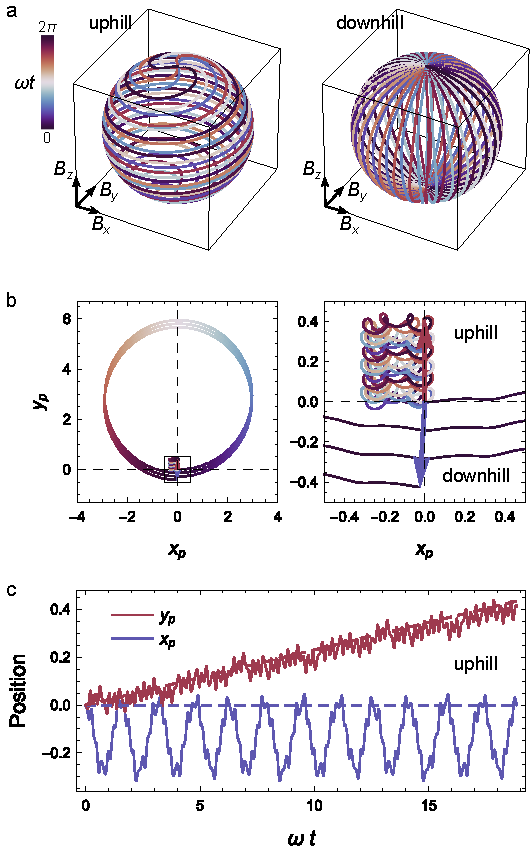
\includegraphics[width=8.5cm]{figures/5ModelDriven.pdf}
    \caption{(a) Two periodic fields $\ve{B}'(\omega t)$ from equation (\ref{eq:field}) designed to drive particle motion uphill (left) and downhill (right).  The uphill field has parameters $m=4$ and $b=40$; the downhill field has parameters $m=28$ and $b=0$. (b) Numerically computed particle trajectories in the $xy$ plane over three oscillation cycles using the fields in (a). The uphill field causes the particle to ``wiggle'' erratically with an average velocity of $\langle U_y\rangle = 0.022\omega$. The downhill field drives the particle around large circular orbits with a net velocity $\langle U_y\rangle = -0.023\omega$. Here, the dimensionless frequency is $\omega=0.005$; the incline angle is $\alpha=0.2$ rad; the hydrodynamic parameters are $\lambda=1.87$ and $\kappa=0.108$. (c) Particle dynamics  computed numerically (solid curves) compared favorably with the time-averaged dynamics (dashed lines) predicted by equation (\ref{eq:Uy21}). Data correspond to the uphill trajectory in (b).}
    \label{fig:ModelDriven}
\end{figure}

According to equation (\ref{eq:Uy21}) for the migration velocity, we can select large values of $b$ to drive particle motion uphill or large values of $m$ to drive particle motion downhill.  Figure \ref{fig:ModelDriven} illustrates these two scenarios for dimensionless frequency $\omega=0.005$ and incline angle $\alpha=0.2$.  During steady migration up the inclined surface, the particle zigzags back and forth in the $x$ direction ($m$ times per cycle) as it wiggles its way along the $y$ direction (Fig.~\ref{fig:ModelDriven}b,c). Steady migration down the inclined surface is accomplished using a qualitatively different motion whereby the particle rolls along nearly circular orbits (Fig.~\ref{fig:ModelDriven}b). In both examples, the approximate migration velocity of equation (\ref{eq:Uy21}) agrees well with the steady motions computed numerically (Fig.~\ref{fig:ModelDriven}c).  More generally, the validity of the perturbation expansion requires that $|\dot{\ve{B}}| \ll 1$ such that the field varies slowly relative to the particle relaxation rate. For large $m$ or $b$, this condition implies that $\omega\ll (m^2+b^2)^{-1/2} \ll 1$.

In dimensionless units, the uphill migration velocity for $b\gg m$ can be approximated as 
\begin{equation}
    \langle \ve{U} \rangle \approx C_b(\lambda) \kappa \alpha b^2\omega^2 \ve{e}_y 
\end{equation}
To maximize the migration velocity, one should increase the product $b\omega$ as much as possible while maintaining the requirement that $b\omega \ll 1$.  Assuming that $b\omega\approx 0.3$, the characteristic migration velocity in \emph{dimensional} units is
\begin{equation}
    \langle \ve{U} \rangle \approx \frac{0.09 C_b Y_B}{6\pi (Y_A Y_C-Y_B^2)} \frac{m B_0\alpha}{\eta a^2} \ve{e}_y \approx (2.37\times10^{-5}) \frac{m B_0 \alpha}{\eta a^2}  \ve{e}_y
\end{equation}
where the second expression assumes a surface separation of $\delta=0.01a$. \kbnote{For Wenjie's system,\cite{Fei2018} $m=2.9\times10^{-14}$ A m$^2$, $B_0=10$ mT, $\eta=0.001$ Pa s, and $a=2~\mu$m, which gives a prefactor of 1.8 $\mu$m/s per radian of incline. When the magnetic moment scales as the volume of the particle, a larger particle would help.  Please estimate for the larger particles you are using.  Compare to gravitational velocity.}
%Gradient-driven motions of ferromagnetic rollers can drive migration at modest speeds of XXX $\mu$m/s. In making 

%%%%%%%%%%%%%%%%%%%%%%%%%%%%%%%
%%%%%%%%%%%%%%%%%%%%%%%%%%%%%%%
\subsection{Data-driven Design}

\begin{outline}
    \1 Motivation
        \2 Expanding the design space of possible fields enables the discovery of more effective strategies for topotaxis.
        \2 The use of numerical solutions (not analytical approximations) allows one to operate within a wider range of conditions (e.g., higher frequencies).
        \2 This methodology can be extended to design problems for which accurate models are unavailable.
\end{outline}


We consider periodic magnetic fields $\ve{B}(t)$ with a fundamental frequency $\omega$ and $N$ harmonics
\begin{equation}
    \ve{B}'(t) = \sum_{n=0}^N \ve{b}'_n e^{i n \omega t}
\end{equation}
where $\ve{b}'_n$ are constant vectors. Only the real part of the Fourier series is physically meaningful; the prime symbols remind us that the field is specified in the world coordinates.  This $6N+3$ dimensional design space is constrained by equation (\ref{eq:rotation}), which ensures that the field has $m$-fold rotational symmetry about the $z'$-axis. For $n=0$, this constraint implies that $\ve{b}'_0 = c_0 \ve{e}'_{z}$ where $c_0$ is a real constant. The first harmonic has Fourier coefficients of the form 
\begin{equation}
    \ve{b}'_1 = c_1 \begin{bmatrix} 1\\-i\\0\\ \end{bmatrix} + d_1 \begin{bmatrix} i\\1\\0 \end{bmatrix}
\end{equation}
where $c_1$ and $d_1$ are  real constants that specify the magnitude and phase of a rotating field in $x'y'$ plane. More generally, there exist rotationally symmetric contributions to the field for $n=0, 1, k m-1, k m, k m + 1$  where $k= 1,2,\dots$ is a positive integer. For higher harmonics equal to a integer multiple of the symmetry order $m$, the Fourier coefficients have the form
\begin{equation}
    \ve{b}'_{n} = c_{n} \begin{bmatrix} 0\\0\\1 \end{bmatrix} + d_{n} \begin{bmatrix} 0\\0\\i \end{bmatrix} \quad \text{for} \quad n=km
\end{equation}
Neighboring harmonics with $n=km\pm 1$ have Fourier coefficients of the form
\begin{equation}
    \ve{b}'_{n} = c_{n} \begin{bmatrix} 1\\\mp i \\0\end{bmatrix} + d_{n} \begin{bmatrix} \pm i\\1\\0 \end{bmatrix} \quad \text{for} \quad n=km \pm 1
\end{equation}
To limit the size of our design space, we fix the number of higher harmonics to $N=m+1$. In this way, the full $6N+3$ dimensional design space is reduced to nine dimensions (namely, $c_0$, $c_1$, $d_1$ $c_{m-1}$, $d_{m-1}$ $c_{m}$, $d_{m}$, $c_{m+1}$, and $d_{m+1}$). As the phase of the driving field is not important, we set $d_1=0$ without loss of generality. Moreover, as the field has rotational symmetry about the $z'$ axis, rotation of the field about that axis by any angle is not important; we can therefore set $c_{0}=0$. Each of the seven remaining parameters is bounded on the range $[-1,1]$ to constrain the magnitude of the field. 
%Figure XXX illustrates one possible magnetic field with $m=5$ fold symmetry.

Within this design space, we seek fields that minimize the following objective function
\begin{equation}
    L(\ve{d},\omega) = -\frac{\Delta_y}{1 + (10 \Delta_x/\Delta_y)^2} \label{eq:objective}
\end{equation}
where $\ve{d}$ is the design vector containing the value of the seven field parameters, and $\veS{\Delta}$ is the particle displacement during one oscillation cycle at the periodic steady-state.  This function favors rapid particle motion up the inclined surface in the positive $y$ direction (Fig.~\ref{fig:Coordinates}); the factor of 10 sets the relative importance of the magnitude and orientation of the displacement $\veS{\Delta}$. Here, the displacement $\veS{\Delta}$ is computed numerically by integrating equations (\ref{eq:theta})--(\ref{eq:Uy}) in time for a specified field. In principle, this information could also be obtained from an automated experiment without reference to a physical model. We specify the frequency as $\omega=1/2 m$ to match the time-scale of the field with that of particle relaxation; however, it can also be treated as a design variable.  We use XXX optimization to identify designs $\ve{d}$ that minimize the objective function (\ref{eq:objective}).

Figure XXX shows the results of this procedure.

\kbnote{Yong, please work on this section. In the data-driven approach, we select fields from a suitable design space (as we did previously) and measure some observed quantity (e.g., particle displacement in $x$ and $y$ directions after a prescribed number of cycles). Here, this observed quantity is computed numerically from the model; however, it might also be obtained from experiment. We can hold the frequency constant or treat it as a design variable.  Knowledge of the parameters $\lambda$ and $m$ is used only in the simulation of observables.  We define an objective function and seek the design that maximizes the objective function. We then discuss the ``solutions'' obtained by this approach and how they differ from the model-driven designs. }



%%%%%%%%%%%%%%%%%%%%%%%%%%%%%%%
%%%%%%%%%%%%%%%%%%%%%%%%%%%%%%%
%%%%%%%%%%%%%%%%%%%%%%%%%%%%%%%
\section{Conclusions}
